\documentclass[letterpaper,10pt,twocolumn,titlepage]{article}

\usepackage{graphicx}                                        
\usepackage{amssymb}                                         
\usepackage{amsmath}                                         
\usepackage{amsthm}                                          

\usepackage{alltt}                                           
\usepackage{float}
\usepackage{color}
\usepackage{url}

\usepackage{balance}
\usepackage[TABBOTCAP, tight]{subfigure}
\usepackage{enumitem}
\usepackage{pstricks, pst-node}

\usepackage{geometry}
\usepackage{listings}
\geometry{textheight=8.5in, textwidth=6in}

%random comment

\newcommand{\cred}[1]{{\color{red}#1}}
\newcommand{\cblue}[1]{{\color{blue}#1}}

\usepackage{hyperref}
\usepackage{geometry}

\def\name{Balaji Ramani}

%% The following metadata will show up in the PDF properties
\hypersetup{
  colorlinks = true,
  urlcolor = black,
  pdfauthor = {\name},
  pdfkeywords = {cs311 ``operating systems'' files filesystem
I/O},
  pdftitle = {CS 311 Project 1: UNIX File I/O},
  pdfsubject = {CS 311 Project 1},
  pdfpagemode = UseNone
}



\begin{document}
\title{CS311: Operating Systems I - Assignment 1}
\author{Balaji Ramani}
\date{Jan 21, 2012}
\maketitle
\section{Commit logs}
\begin{center}
  \begin{tabular}{ | l | l | l | }
    \hline
    Time & Message & No of files \\ \hline
	2012/01/23 20:37 & minor changes to eps file - final
commit & 2 \\ \hline
    2012/01/21 23:44 & adding images to latex as eps and make
file changes & 6 \\ \hline
    2012/01/21 04:41 & more comments and style & 1 \\ \hline
    2012/01/21 04:21 & comments and styles & 1 \\ \hline
    2012/01/21 03:06 & some changes to the makefile & 1 \\
\hline
    2012/01/21 02:18 & plots using gnuplot & 3 \\ \hline
    2012/01/21 00:47 & vary block size & 1 \\ \hline
    2012/01/20 22:39 & initial commit & 2 \\ \hline
  \end{tabular}
\end{center}
\section{Block size vs Time plot}
\begin{center}
        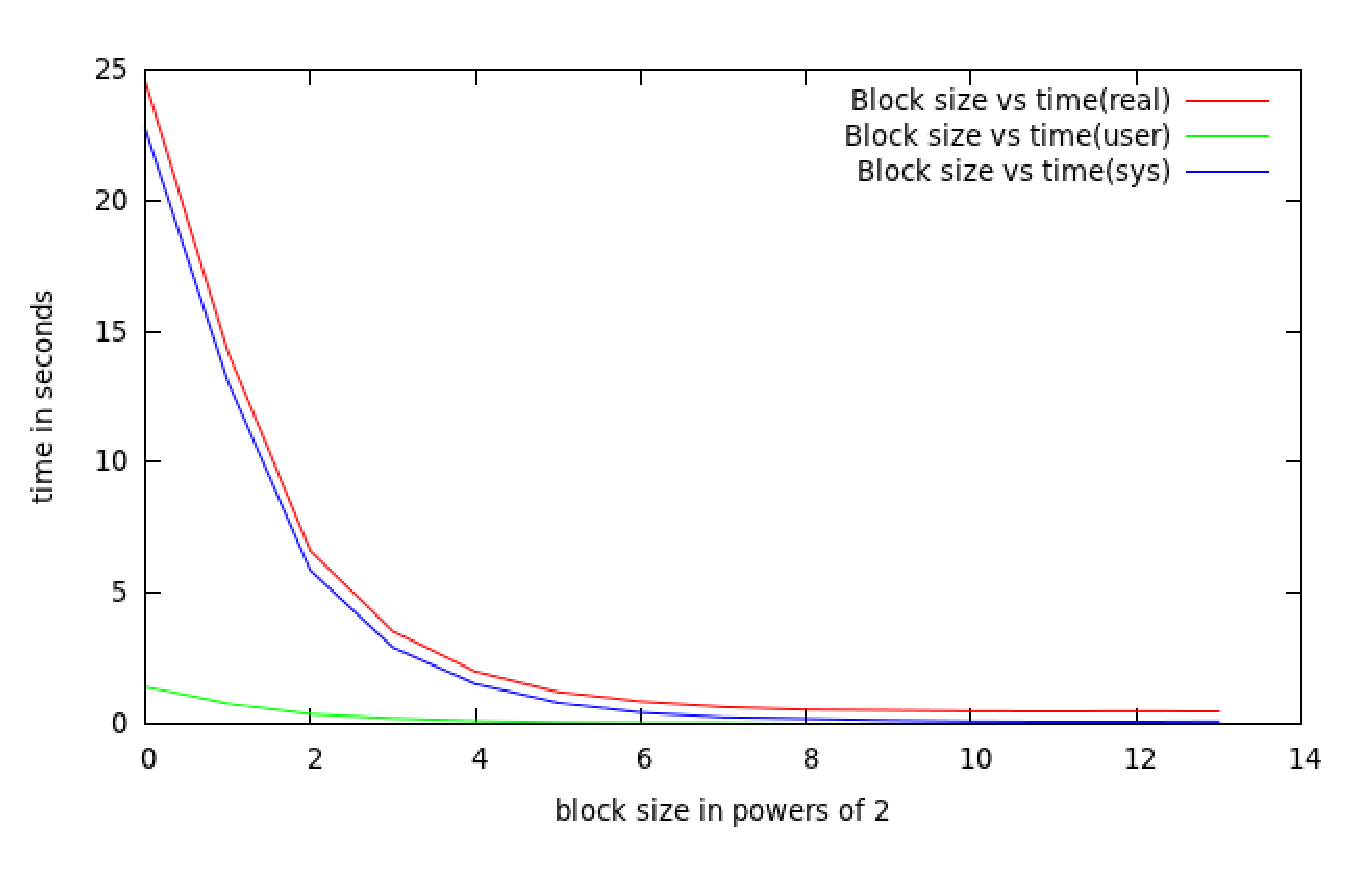
\includegraphics[scale=0.7]{graph.eps}
\end{center}

\end{document}
